\documentclass[thesis=M,czech]{FITthesis}[2012/06/26]

\usepackage[utf8]{inputenc} % LaTeX source encoded as UTF-8

\usepackage{graphicx} %graphics files inclusion
\usepackage{amsmath} %advanced maths
\usepackage{amssymb} %additional math symbols

\usepackage{dirtree} %directory tree visualisation

% % list of acronyms
\usepackage[acronym,nonumberlist,toc,numberedsection=autolabel]{glossaries}
\iflanguage{czech}{\renewcommand*{\acronymname}{Seznam pou{\v z}it{\' y}ch zkratek}}{}
\makeglossaries

\newcommand{\tg}{\mathop{\mathrm{tg}}} %cesky tangens
\newcommand{\cotg}{\mathop{\mathrm{cotg}}} %cesky cotangens

% % % % % % % % % % % % % % % % % % % % % % % % % % % % % % 
% ODTUD DAL VSE ZMENTE
% % % % % % % % % % % % % % % % % % % % % % % % % % % % % % 

\department{Katedra softwarového inženýrství}
\title{Umístění dat na výpočetní uzly minimalizující datové přenosy v databázi HBase}
\authorGN{Miroslav} %(křestní) jméno (jména) autora
\authorFN{Hrstka} %příjmení autora
\authorWithDegrees{Bc. Miroslav Hrstka} %jméno autora včetně současných akademických titulů
\supervisor{Ing. Adam Šenk}
\acknowledgements{Doplňte, máte-li komu a za co děkovat. V~opačném případě úplně odstraňte tento příkaz.}
\abstractCS{V~několika větách shrňte obsah a přínos této práce v~češtině. Po přečtení abstraktu by se čtenář měl mít čtenář dost informací pro rozhodnutí, zda chce Vaši práci číst.}
\abstractEN{Sem doplňte ekvivalent abstraktu Vaší práce v~angličtině.}
\placeForDeclarationOfAuthenticity{V~Praze}
\declarationOfAuthenticityOption{4} %volba Prohlášení (číslo 1-6)
\keywordsCS{Nahraďte seznamem klíčových slov v češtině oddělených čárkou.}
\keywordsEN{Nahraďte seznamem klíčových slov v angličtině oddělených čárkou.}

\begin{document}

% \newacronym{CVUT}{{\v C}VUT}{{\v C}esk{\' e} vysok{\' e} u{\v c}en{\' i} technick{\' e} v Praze}
% \newacronym{FIT}{FIT}{Fakulta informa{\v c}n{\' i}ch technologi{\' i}}

\begin{introduction}
	uvod moji prace :P
\end{introduction}

\chapter{Současný stav a použité technologie}
V této úvodní kapitole je dán prostor pro seznámení s technologiemi a projekty, se kterými se bude buď přímo pracovat nebo je jejich znalost pro pochopení problematiky nezbytná. Jako první je představen projekt Hadoop\textsuperscript{TM} od firmy Apache\textsuperscript{TM} jako celek. Vše, co bude v této práci představeno, se bude odehrávat v rámci tohoto ekosystému. Pro porozumění základní myšlenky projektu Hadoop je také nezbytné vysvětlit programovací model MapReduce. Po uvedení celého Hadoopu jsou detailněji uvedeny produkty, které jsou součástí tohoto ekosystému a se kterými se bude dále pracovat. Jedná se především o databázový systém HBase a také souborový systém HDFS, který je v celém modelu využíván. 


\section{Hadoop Ekosystém}
Apache Hadoop je framework který sdružuje projekty  vyvíjející software  po spolehlivé, škálovatelné a paralelní zpracování dat na počítačových clusterech. Je založen na dvou stěžejních  technologiích pocházejících od firmy Google  a to na distribuovaném souborovém systému Google File System (GFS) a na algoritmu MapReduce\cite{HadoopDum}. Všechny klíčové projekty v systému Hadoop jsou združeny  pod Apache Software foundation, která poskytuje podporu pro tyto projekty. Jedná se o open.source software a Všechny komponenty jsou psány v Jprogramu Java.

\subsection{Základní principy}
Podstata Hadoopu spočívá v uložení dat na velkém množství výpočetních úzlů spojených do clusterů. Většinou se jedná o běžný hardware. Na těchto uzlech jsou data uložená ve vlastním souborovém Systému HDFS. K výpočtům nad clusterem se využívá princip Mapreduce, který bude osvětlen v následující kapitole. Systém Hadoop je charakteristický především následujícími vlastnostmi, které ho odlišují od klasických databázových systémů.

\begin{description}

  \item[Horizontální škálovatelnost a komoditní hardware] \hfill \\
  Pro objemy dat, jimiž by se měl Hadoop při svém zpracovávání primárně zabývat, je poměrně složité a především velmi drahé dosáhnout dostatečné škálovatelnosti pomocí vertikálního škálování, tedy přidávání výkonu a zdrojů ke stávajícím výpočetním uzlům. Proto Hadoop využívá horizontálního škálování. Díky horizontálnímu škálování se nabízí využití komoditního hardwaru namísto specializovaných výpočetních uzlů. Systém tedy běží na velkém množství samostatných počítačů spojených do clusteru.
  \item[Řešení selhání hardwaru] \hfill \\
   S předchozím bodem úzce souvisí řešení případných výpadků jednotlivých uzlů. Kvůli velkému počtu výpočetních uzlů a díky použití běžného hardware jsou výpadky poměrně časté. Hadoop je ale navržen tak, že se nesnaží tyto výpadky minimalizovat, ale počítá s nimi. Data jsou dostatečně replikovány a pokud dojde k výpadku při zpracování dat, je přerušená úloha provedena na jiném uzlu obsahující danou replikaci a zároveň je automaticky vytvořena nová záloha dat. Defaultně je zálohovací faktor nastaven na {\texttt{3}} , tedy každý soubor je uložen ve třech kopiích na různých výpočetních uzlech.  
  \item[Přenášení kodů k datům] \hfill \\
  Kvůli velkým objemům dat a poměrně nízké propustnosti sítě spojující jednoltivé výpočetní uzly v clusteru je velmi výhodné namísto rozesílání dat na jednotlivé výpočetní uzly rozesílat na ně pouze kód výpočtu a minimalizovat tak přesuny dat mezi uzly. Na každém uzlu je tak vykonán výpočet pokud možno s lokálními daty.
  \item[Abstrakce od distribuovaných a paralelních aplikací] \hfill \\
  Hadoop se snaží co nejvíce odstínit vývojáře Hadoop aplikací od řešení zpracování pomocí paralelního a distribučního zpracovaní. Proto poskytuje poměrně jednoduché a dobře definované rozhraní pro jednotlivé komponenty. Při práci s těmito rozhraními tak není nutné řešit, jak se bude kód v clusteru distrubuovat ani další záležitosti spojené s paralelním zpracováním a dovoluje se zaměřit na business logiku aplikace. Cenou za toto zjednodušení je pak právě omezené rozhraní bez možnosti detailnějšího nastavení. 

\end{description}

\subsection{MapReduce}
MapReduce je programovací paradigma určené k provádění výpočtů, které by za normálních okolností trvaly značné množství času a to zejména z důvodů velkého množství dat. Tyto výpočty se pak snaží dokončit v přijatelném časovém horizontu. Princip byl poprvé představen v roce 2004 v  práci pro firmu Google jako jedno z opatření pro zvládání obrovského množství dat, se kterým se museli potýkat.

V MapReduce jsou data modelována do párů klíč/hodnota. Tento formát je velmi jednoduchý, přesto se dají téměř všechny údaje takto prezentovat. Tato jednoduchá datová struktura tak umožňuje snadné zpracování dat efektivním způsobem. Klíč a hodnota může být cokoliv. Může se jednat o řetězce, čísla nebo komplexní struktury.

Mapreduce se skládá ze dvou hlavních fází, mapovací fáze a redukční fáze. Nejdříve je spuštěna mapovací funkce, která je dále spočtena nad jednotlivými prvky z množiny uspořádaných dvojic (klíč, hodnota), jež produkuje přechodné klíče a hodnoty.\cite{HadoopDG}
Poté se všechny tyto přechodné hodnoty asociované se stejným klíčem seskupí a pošlou se do redukční fáze. Redukční fáze přijme na vstupu klíč a související množinu hodnot. Jako výstup je pak množina uspořádaných dvojic, která splňuje zadaná kritéria.

Jak vstupní data, tak mezivýsledky i finální výsledky jsou ve formátu klíč/hodnota. Jak je vidět na obrázku \ref{fig:mapred} probíhají mapovací a redukční fáze paralelně. Z diagramu je také zřejmé, že mezi mapovací fází a fází přeskupování(shuffling) dochází k přenosu průběžných výsledků mezi jednotlivými výpočetními uzly. Právě optimalizací přesunů v těchto místech se bude zabývat hlavní část této práce. 
MapReduce je také často popisována funkcí: 

\begin{eqnarray}
	map: (k_1, v_1) \rightarrow  list(k_2, v_2) \nonumber \\
	reduce: (k_2, list(v_2)) \rightarrow list(k_3, v_3) \nonumber 
\end{eqnarray}

\begin{figure}\centering
	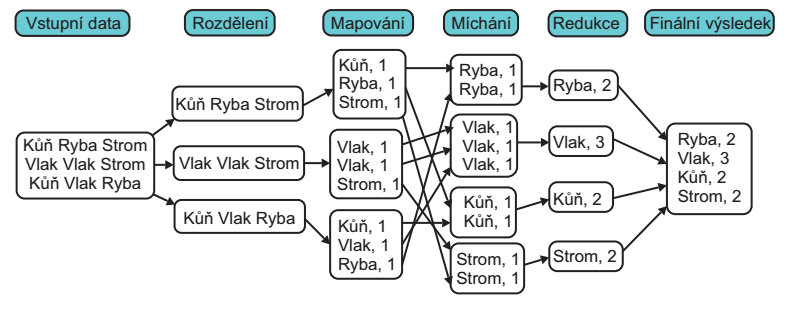
\includegraphics[width=1\textwidth, angle=0]			{files/MapReduce}
	\caption[Diagram MapReduce procesu]{Diagram MapReduce procesu}\label{fig:mapred}
\end{figure} 


\subsection{Hadoop Ekosystém}
Následující kapitola je určena k seznámení s ekosystémem Hadoop, který kromě základních projektů MapReduce a HDFS obsahuje množství dalších projektů. Složení ekosystému se ale liší v závoslosti na konkrétní distribuci Hadoopu. Je sice možné zvolit si tyto aplikace podle svého výběru a využít přímo zdroje od firmy Apache, ale  v praxi se využívají spíše již částečně nakonfigurované distribuce. které navíc nabízejí i možnost placené podpory. Mezi největší hráče na trhu patří distribuce od firem Cloudera, MapR a Hortonworks.\cite{CLOUDERA} Pro účely této práce byla vybrána distribuce Cloudera, protože se jedná o open-source projekt a také kvůli největšímu podílu na trhu.\ref{fig:eko}  

\begin{figure}\centering
	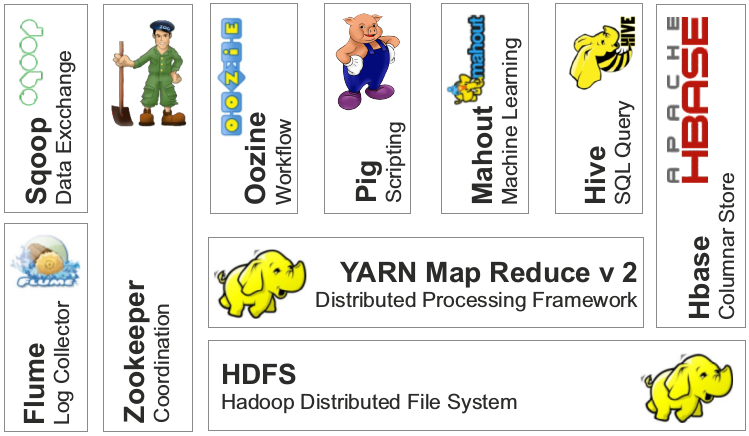
\includegraphics[width=1\textwidth, angle=0]{files/HadoopEco}
	\caption[Hadoop Ekosystém]{Hadoop Ekosystém}\label{fig:eko}
\end{figure}

\paragraph{Nástroje pro vývoj}
\begin{description}
\item[YARN] \hfill \\
YARN je klíčovým prvkem Hadoop 2. Někdy je také zvaný  MapReduce v2. Jedná se o distribuovaný operační systém, který odděluje řízení zdrojů a řízení kapacit od zpracovávající komponenty. To umožňuje  podporovat větší škálu přístupů ke zpracování dat a širší pole aplikací.

\item[Hive] \hfill \\
Hive umožňuje dotazování nad velkými datasety uloženými v distribuovaném systémua také jejich řízení. Poskytuje mechanismus k vytvoření struktury nad těmito daty a následně nad daty provádět dotazy v SQL-like  jazyku HiveQL. Kromě toho umožňuje také využití klasického map/reduce postupu v případech, kdy není výhodné použít HiveQL. 

\item[Pig] \hfill \\
Pig poskytuje prostředí pro zpracování jednoduchého skriptovacího jazyka Pig Latin, ve kterém je přeložen na sérii MapReduce úloh. Pig Latin abstrahuje od MapReduce schématu a nabízí dotazování na vyšší úrovni, podobné jako SQL.

\item[Mahout] \hfill \\
Mahout je škálovatelná knihovna pro strojové učení. Jsou v ní implementovány algoritmy pro clustering, klasifikaci a kolaborativního filtrování optimalizované pro běh v prostředí Hadoopu.
\end{description}
\paragraph{Ukládání dat a správa metadat}
\begin{description}
\item[HDFS] \hfill \\
Jedná se o distribuovaný souborový systém navržený  pro provoz na komoditním hardwaru ve velkých datových skladech, souborový systém HDFS bude detailněji představen v následující kapitole.

\item[HBase] \hfill \\
Hbase je sloupcově orientovaný databázový systém, který běží nad HDFS. Nepodporuje strukturovaný dotazovací jazyk a poskytuje prakticky pouze CRUD operace. HBase bude stejně jako HDFS představen detailněji v následujících kapitolách.
\end{description}
\paragraph{Nástroje pro řízení}
\begin{description}
\item[ZooKeeper] \hfill \\
Poskytuje provozní služby pro Hadoop cluster. Jedná se o distribuované konfigurační, synchronizační služby a o jmenné registry pro distribuovaný systém. 

\item[Oozie] \hfill \\
Aplikace používaná pro plánování Hadoop úloh. Je složena ze dvou hlavních částí. V první části se ukládají a spouštějí různé typy hadoop úloh (Mapreduce, Pig, Hive, atd.) a z části, která koordinuje běh daných úloh na základě předdefinovaných plánů a dostupnosti dat.
\end{description}

\paragraph{Získávání a agregace dat}
\begin{description}
\item[Sqoop] \hfill \\
Nástroj sloužící k efektivnímu přenosu dat z relačních databází do Hadoopu k dalšímu zpracování. Zpracovat tyto data pak může buď MapReduce úloha nebo jiný nástroj (Hive, Pig) Je také možné data zložít do HBase databáze.
\item[Flume] \hfill \\
Služba pro efektivní získávání, agregování a přesouvání velkého množství streamovaných dat do HDFS. Typicky se používá k ukládání logů z jednoho zdroje (webové logy, bankovní logy) a agreguje je v HDFS pro pozdější zpracování.
\end{description}

\section{HDFS}
Hadoop Distributed File Systém (HDFS) nabízí způsob skladování velkých souborů na více samostatných počítačích, který je rozdílný oproti klasickému přístupu skladování dat na jednom stroji s dostatečnou diskovou kapacitou. HDFS je navržen na základech Google File Systemu (GFS) a běží na nativním filesystému (Ext3, Ext4,XFS). HDFS je určen pro skladování především velkých souborů (100 MB a více) v menším počtu (řádově miliony) a k ukládání streamovaných dat. Systém dále není vhodný pro soubory, u nichž se očekává časté upravování a to protože je možné připisovat data pouze na konec souboru. Systém je odolný proti chybám v replikaci a výpadkům v distribuci dat.\cite{HDFSWEB}

HDFS umožňuje, stejně jako většina běžných souborových systému, operace čtení, zápisu a mazání souborů a vytváření a mazání adresářů. Vždy, když je načten nový soubor do HDFS je zreplikován do žádoucího počtu, který určuje replikační faktor (defaultní hodnota je 3) a rozdělen do bloků dat o fixní délce (defaultně 64MB). Tyto bloky jsou pak rozdistribuovány a uloženy  ve vybraných uzlech clusteru určených pro skladování, tzv. DataNodes viz.\ref{fig:hdfs} . V HDFS se informace o souborech neukládají společně s daty, ale jsou uloženy na vyhrazeném serveru nazývaném NameNode. Při přístupu k datům klient nejdříve zadá požadavek na data na NameNode, který následně vrátí adresy databloků s požadovanými daty. NameNode tedy přípo nemanipuluje s daty.

\begin{figure}\centering
	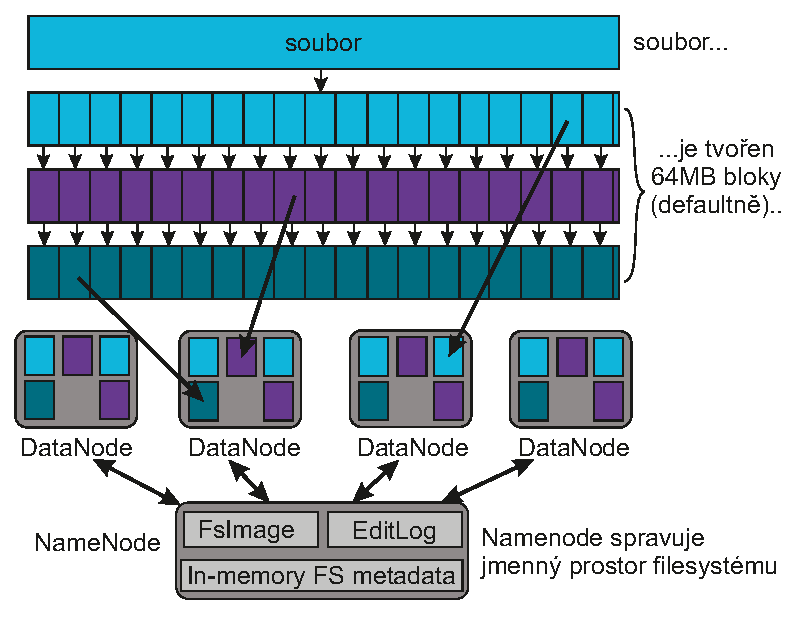
\includegraphics[width=0.8\textwidth, angle=0]{files/hdfs}
	\caption[Diagram uložení souboru v systému HDFS]{Diagram uložení souboru v systému HDFS}\label{fig:hdfs}
\end{figure}

NameNode uchovává a poskytuje strom jmenného prostoru a adresy fyzického umístění bloků ve své operační paměti. Dále ukládá perzistentní záznam těchto adres (kontrolní bod) a registr modifikací (žurnál) pro zotavení z havárie v nativním systému souborů hostitelského počítače. HDFS umožňuje i  vytvoření kopie kontrolního bodu a žurnálu na další výpočetní uzel nazývaný SecondaryNameNode. Ten pak slouží jako záloha dat serveru NameNode  (nenahrazuje tedy funkci primárního NameNode v případě výpadku, pouze poskytuje data pro jeho obnovu). Ve verzi Hadoop 2+ je už možné mít Standby NameNode, který v případě výpadků může primární NameNode plně a okamžitě nahradit. 

Přistupovat k HDFS je možné přímo a to přes nativního klienta nebo pomocí Java nebo C++ API. Dále je možný přístup přes proxy server podporující REST, Thirft a Avro server.

\section{HBase}
Jedná se o sloupcově orientovanou databázi, někdy označovanou jako Hadoop databáze. HBase podporuje náhodné real-time CRUD operace (narozdíl od HDFS). Je primárně navržená pro uchovávání velkých tabulek o miliardách řádků a milionech sloupcích a jedná se o NoSQL databázi. Nepodporuje tedy přístup založený na SQL jazycích ani relační model. Stejně jako HDFS se vyznačuje jednoduchým klientem a Java API. HBase je založena na projektu Bigtable od Googlu a stejně jako byl Bigtable postaven nad GFS je HBase postavena nad HDFS.\cite{HbaseDG}

HBase nebyla zavedena za účelem nahrazení klasických RDBMS a ani k tomuto účelu není využívána. HBase je výhodné použít, jak již bylo řečeno, v případě rozsáhlých tabulek. Výborné výsledky vykazuje při vykonávání jednotlivého náhodného výběru z databáze a při vyhledávání dle klíče. Hbase je také vhodným řešením v případě, že jednotlivé řádky tabulky jsou velmi různorodé a v případě řidkých databází, kdy je velký počet sloupců a většina z nich obsahuje nulovou hodnotu. Nevhodné využití je pak právě pro suplování úloh pro tradiční RDBMs jako jsou transakční aplikace nebo relační analýza.\cite{HBaseWEB}

\subsection{Data model HBase}


Data v databázi HBase jsou uložena v tabulkách. Jednotlivé tabulky obsahují řádky. Na každý řádek odkazuje unikátní klíč. Jako hodnota klíče se bere bitové pole. Klíč u HBase tedy může být cokoli, string, long nebo vlastní datová struktura. Každý řádek je složen ze sloupců, které jsou sdruženy do rodin (column families). Tyto rodiny sloupců jsou definovány staticky při vytváření databáze narozdíl od samotných sloupců, které se mohou přidávat libovolně. Data jako taková jsou pak uložena v buňkách. Tyto buňky jsou identifikovány pomocí řádku, rodiny, sloupce a časovou značkou(timestamp). Obsah každé buňky je pak uchováván také jako pole bitů. Data v buňkách jsou navíc verzovány. Každá buňka defaultně uchovává poslední tři zadané hodnoty s tím, že pokud není v dotazu specifikována konkrétní verze, vrací vždy tu nejmladší. Řádky jsou v každé tabulce seřazeny lexikograficky podle svého klíče.

\begin{figure}\centering
	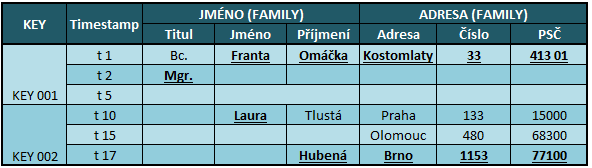
\includegraphics[width=1\textwidth, angle=0]{files/hbase}
	\caption[Datový model HBase]{Datový model HBase}\label{fig:hbase}
\end{figure}

\subsection{HBase Architektura}
HBase je distribuovaná databáze. Proto je i architektura složitější než u databázích běžících na jednom výpočetním uzlu. HBase musí řešit všechny problémy typické pro distribuované aplikace jako je koordinace a řízení vzdálených procesů, blokování, distribuce dat a příliš velká síťová komunikace. HBase však k tomuto z velké části využívá služeb v rámci Hadoop a Zookeeper. Následující obrázek \ref{fig:hbasearch} popisuje hlavní architektonické komponenty HBase.
\begin{figure}\centering
	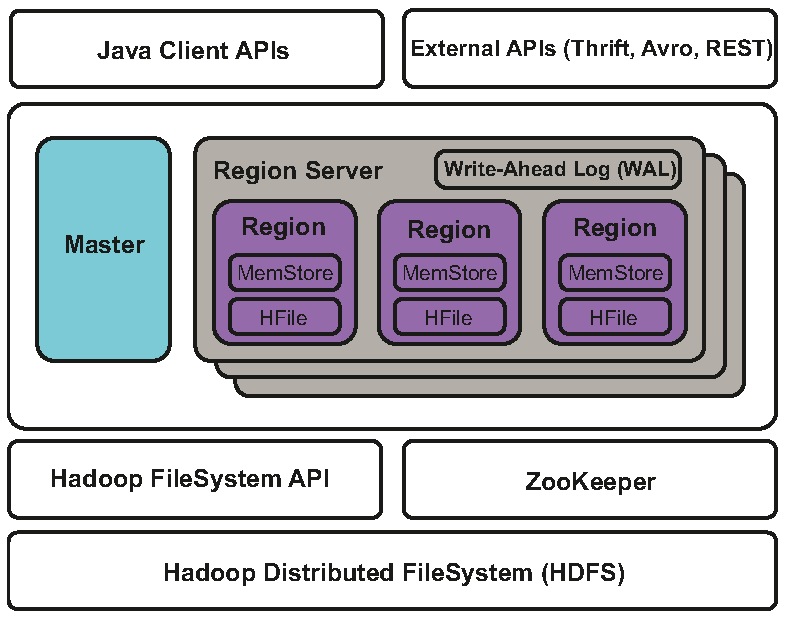
\includegraphics[width=0.8\textwidth, angle=0]{files/hbase-architecture}
	\caption[Architektura databáze HBase]{Architektura databáze HBase}\label{fig:hbasearch}
\end{figure}

Jednotlivé tabulky jsou složeny z regionů. Region je vždy určitý rozsah řádků uložený pohromadě. Protože jsou řádky v databázi ukládány v lexikografickém pořádí, je nutné počítat s tím, že se velikost těchto rozsahů, tedy regionů, bude v čase měnit. Proto se v případě, kdy velikost regionu překročí stanovenou hranici, rozdělí region na dva přesně v půli podle prostředního klíče. Naopak v případě, kdy se regiony příliš zmenší, dojde k jejich sloučení. Regiony jsou uložené v region serverech. Každý region server může obsahovat jeden a více regionů. Region je však vždy jen na jednom serveru. Master server je zodpovědný za správu region serverů. Pro koordinaci se využívá Zookeeper. Na každém regionu je uložen určitý rozsah klíčů. Rozdělení dat do region serverů umožňuje rychlou obnovu v případě pádu region serveru a také ulehčuje load balancing pokud dochází k přetěžování některých serverů. Všechny tyto činnosti včetně rozdělování velkých regionú jsou prováděny automaticky bez zásahu uživatele.

\subsection{Architektura uložiště RDBMS vs HBase}
Dříve než bude uveden detailní pohled na uložení dat v databázi HBase, je na místě popsat základní rozdíl mezi typickou architekturou uložení dat v RDBMS a v HBase. Typické RDBMS ukládá data do struktury B+ Trees oproti tomu HBase a ostatní Big Table architektury využívají Log-Structured Merge Trees.

\subsubsection{B+ Trees}
Jedná se o stromovou datovou strukturu, která vychází z B-stromu. Umožňuje rychlé vkládání, vyhledávání a mazání dat. Záznamy v tabulkách jsou identifikovány za pomoci klíčů. Všechna data jsou uložena jen na listech stromu, oproti klíčům, které jsou uloženy i ve vnitřních uzlech. V implementaci těchto stromů se přidává do všech listů kromě vlastních klíčů i odkaz na následujícího sourozence. To umožňuje velmi efektivní sekvenční prohledávání aniž by výrazněji stoupla paměťová náročnost na uložení stromu, odkaz na sourozence je v obrázku znázorněn červenými políčky \ref{fig:btree}. 

V B+stromech je data-locality dosažená na úrovni stránek, kde stránky odpovídají blokům v jiných systémech. Stránka tak může vypadat například takto:
\begin{itemize}
	\item Odkaz na předchozí stránku
	\item Odkaz na následující stránku
	\item key: A $\rightarrow d_A$
	\item key: B $\rightarrow d_B$
	\item key: C $\rightarrow d_C$
	\item key: D $\rightarrow d_D$
\end{itemize}

Vždy, když se vkládá nový záznam, doplní se daná stránka požadovaným záznamem. Pokud dojde k případu, že stránka už je plná, rozdělí se na 2 poloprázdné stránky a upraví se patřičně rodič těchto stránek. Tímto dochází k fragmentaci dat na disku, kdyz jednotlivé logicky sousedící stránky neleží vedle sebe fyzicky.
\begin{figure}\centering
	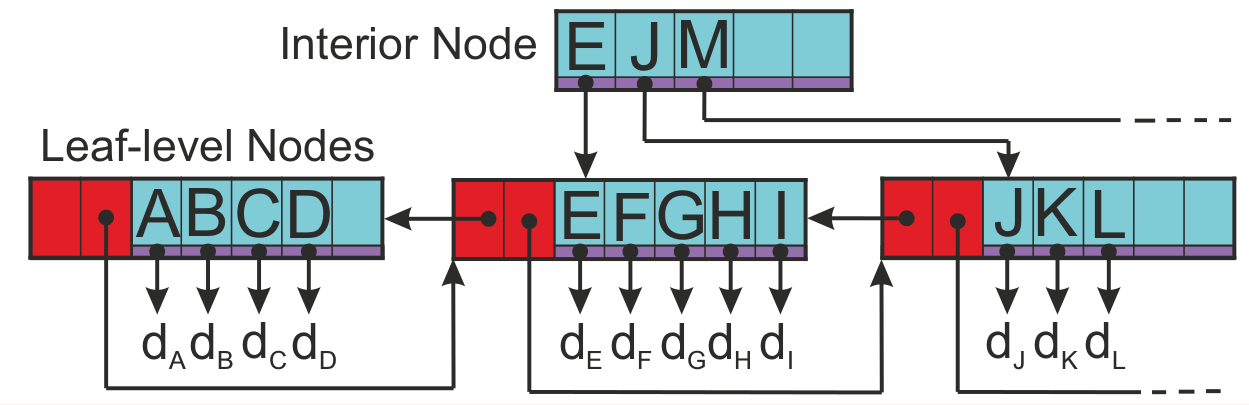
\includegraphics[width=1\textwidth, angle=0]{files/Bplustree}
	\caption[Příklad B+ stromu.]{Příklad B+ stromu. Obsahuje data $d_1$ až $d_7$}\label{fig:btree}
\end{figure}


\subsubsection{Log-Structured Merge Trees}
Log-Structured Merge Trees využívají odlišný způsob. Všechny příchozí data jsou nejprve ukládány v logovacích souborech a to kompletně sekvenčně. Jakmile jsou informace uložené v logu, uloží se data v in-memory uložišti, kde jsou uloženy naposledy upravené záznamy. Vždy, když je k dispozici dostatečný počet záznamů, dojde k zapsání už seřazených dat do uložiště souborů. Po zapsání dat na disk je log soubor smazán. 


Datové soubory jsou pak strukturovány podobně jako B stromy, s tím že jsou optimalizovány pro sekvenční přístup na disku. Všechny uzly stromu jsou zaplněny a uloženy v sigle-page nebo multi-page bloku. Při přidávání dat se uložené data na disku v multi-page blocích spojí s příchozími in-memory daty.\ref{fig:lms}.  Vždy, když data využíjí celou kapacitu bloků, dojde k vytvoření nového.
Postupně se tak zvyšuje počet vytvořených souborů. Tyto soubory jsou pak spojovány do větších celků. Všechny tyto soubory jsou uloženy sekvenčně za sebou a tak je umožněn optimální sekvenční přístup k datům.
Strom může být také rozdělen v případě, kdy je potřeba vložit nové data s klíči mezi ostatními.
Mazání záznamů se provádí dávkově. Každý záznam, který je určený k smazání je označen jako smazaný, a při nahlížení do dat se ignoruje. Při přepisování stránek pak dojde k odstranění těchto záznamů ze stromu.

Z těchto rozdílných přístupů k uložení dat vyplývá, že B+ stromy jsou určeny pro úlohy, kde se očekává častá modifikace již vložených dat, zatímco LSM stromy jsou určeny k ukládání velkého množství dat a jeho následovnému čtení.


\ref{fig:lms}. 

\begin{figure}\centering
	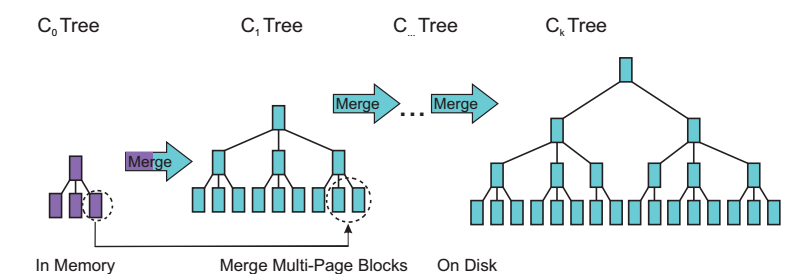
\includegraphics[width=1\textwidth, angle=0]{files/lms}
	\caption[Iterativní Merge Multi-Page bloků v LMS stromu ]{Iterativní Merge Multi-Page bloků v LMS stromu }\label{fig:lms}
\end{figure}

\subsection{Fyzické uložení dat}	
K uložení dat se typicky využívá souborový systém HDFS. Data jsou pak v souboru uložena v souborech nazývaných HFile. HFile má strukturu key-value mapy, kdy klíče jsou uloženy lexikograficky. 




\chapter{Existující řešení optimalizace distribuce dat pro MapReduce}
V této kapitole bude představeno řešení, které poskytl M. Liroz-Gistau et al. ve svém článku Data Partitioning for Minimizing Transfered Data in MapReduce \cite{gistau}. V tomto článku se zaměřují na redukování datových přenosů mezi mapovací a redukční fází. V tomto místě přichází na řadu fáze, kde probíhá míchání přechodných klíčů(shuffle phase). Od tohoto řešení se bude poté odvíjet návrh řešení pro databázi HBase. Protože v předchozích kapitolách už byl vysvětlen princip zpracování dat pomocí Map Reduce, může tato kapitola plynule navázat na tyto poznatky. 

\section{Definice problému}
Nejdříve je zapotřebí fommálně definovat, jaký problém chceme řešit. Mějme tedy sadu MapReduce úloh, které reprezentují typické zatížení systému a sadu vstupních dat. Předpokládejme, že budoucí MapReduce úlohy budou vykonávat podobné úlohy na podobných datech a budou generovat podobné intermediate key (předpokládá se, že v praxi se vykonávají pořád stejné úlohy, jen dochází například ke zvětšování datasetu o nově zapsané data). 

Cílem navrhovaného systému je automatické rozdělení vstupních dat tak, aby u budoucího vykonávání MapReduce úloh byl minimalizován přenos dat mezi jednotlivými uzly v shuffle fázi. Při tomto rozdělování se nebere v úvahu plánování mapovacích a redukčních fází, ale pouze inteligentní rozdělení intermediate klíčů mezi jednotlivé redukční uzly.

	Definujme daný problém formálně. Mějme vstupní data pro MapReduce úlohu $job_\alpha$ složená z jednotlivých souborů $D = \{d_1, ..., d_n\}$, které jsou rozděleny do  množiny bloků (chunks) $C = \{c_1, ..., c_p\}$. Funkce $loc : D \rightarrow C$ přiřazuje data do bloků. Nechť  $job_\alpha$ je složen z $M_\alpha = \{m_1, ..., m_p\}$ mapovacích úloh a $R_\alpha = \{r_1, ..., r_q\}$ jsou redukční úlohy. Předpokládejme, že každá mapovací úloha $m_i$ zpracuje blok $c_i$. Nechť  $N_\alpha = \{n_1, ..., n_s\}$ je množina výpočetních uzlů použitých pro provedení úlohy. $node(t)$ reprezentuje výpočetní uzel, kde se vykonává úloha $t$.

Nechť $I_\alpha = \{i_1, ..., i_m\}$ je množina intermediate párů klíč-hodnota produkovaných mapovací fází jako je $map(d_j) = \{i_{j_1}, ..., i_{j_t}\}$. $k(i_j)$ reprezentuje klíč z intermediate páru $i_j$ a $size(i_j)$ reprezentuje celkovou velikost v bytech. Definujeme $output(m_i) \subseteq I_\alpha$ jako množinu intermediate párů produkovaných mapovací úlohou $m_i$, tedy $output(m_i) = \bigcup_{{d_j}\in{c_i}} map(d_j)$. Dále definujeme $input(r_i)\subseteq I_\alpha$ jako množinu intermediate párů přiřazených k redukční úloze $r_i$. Funkce $part : k(I_\alpha) \rightarrow R$ přiřazuje intermediate klíč k redukční úloze. 

Nechť $i_j$ je intermediate klíč-hodnota pár, pak  $i_j \in output(m)$ a $i_j \in input(r)$. Nechť $P_{i_j} \in {0,1}$ je proměnná, která se rovná 0 pokud intermediate pár $i_j$ je vyprodukován na stejném výpočetním uzlu jako je následně zpracováván v redukční části a 1 v opačném případě.  

Nechť $W = {job_1, ..., job_w}$ je množina všech úloh. Cílem je pak najít optimální $loc$ a $part$ funkce tak aby $\sum_{job_\alpha \in W} \sum_{i_j \in I_\alpha}  size(i_j)P(i_j) $ bylo minimální.

\section{MR-part}
Pro vyřešení zadaného problému byla navržena technika pojmenovaná MR-Part. Tato technika, za pomocí automatického dělení vstupních souborů, dovoluje využití maximální výhody data-locality při plánování redukčních úloh a výrazně snižuje množství dat, které je potřeba přesunout v shuffle fázi. MR-part se skládá ze tří hlavních fází. Jedná se o fáze Workload Monitoring, Partitioning a Execution and scheduling, tak jak je vidět z obrázku \ref{fig:MR-part}. V první fázi se shromáždují informace o vykonávání jednotlivých MapReduce úloh, které jsou následně zkombinovány. Z těchto informací je vytvořen model zatížení pomocí hypergrafu. V druhé fázi se na vytvořený hypergraf aplikuje dělící algoritmus, který rozdělí data na požadovaný počet bloků a následně jsou vstupní soubory upraveny na základě tohoto rozdělení. V poslední fázi se využije upravených vstupních souborů a za pomoci optimalizace přiřazování redukčních úloh se dosáhne minimalizace přenosu dat v shuffle fázi.

\begin{figure}\centering
	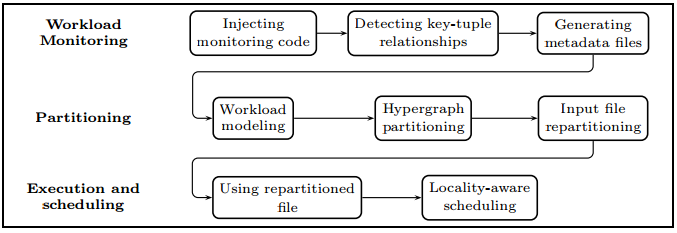
\includegraphics[width=1\textwidth, angle=0]{files/MR-part}
	\caption[MR-part schéma]{MR-part schéma}\label{fig:MR-part}
\end{figure}

\subsection{První fáze - Workload Characterization}
Pro zajištění minimalizace přenosů mezi výpočetními uzly při přechodu z mapovací do redukční fáze je nejdříve zapotřebí zjistit, jaké páry hodnot se generují pro vstupní data a následně je vhodně seskupit. K tomu dochází v monitorovací a kombinační části první fáze.
\paragraph{Monitoring}
Nejprve je zapotřebí získat potřebná data z typických MapReduce úloh, u kterých se očekává jejich častější vykonávání. K zachycení těchto dat se využívá třída  \texttt{RecordReader} \footnote{\texttt{RecordReader} je třída, která parsuje vstupní soubor a generuje vstupní páry. Každý datový formát má jiný \texttt{RecordReader}. Soubory tedy obvykle používají stále stejný.} , která je rozšířená o  monitorovací funkci. Monitorovací funkce unikátně identifikuje vstupní páry klíč-hodnota a jejich pozici ve vstupních datech. Pro každou mapovací úlohu se tek vytvoří soubor s metadaty. Vždy, když je načten nový blok s daty, je zároveň vytvořen i nový soubor, obsahující informace o bloku. Následně je iniciován record counter(rc). Pokaždé kdy je načten vstupní pár, inkrementuje se counter o 1. Poté pokud dojde k vytvoření vstupního páru, je vygenerován pár (k, rc). Po dokončení zpracování bloku dat jsou takto vygenerované páry uloženy do již vytvořeného souboru ve formátu $\langle k,\{rc_1, ..., rc_n\}\rangle$.
\paragraph{Combination}
Následující fáze již neběží zároveň s jinými úlohami, ale pustí je uživatel ideálně v čase, kdy systém není vytížen jinými výpočty. V kombinační fázi se shromáždí a zkombinují metadata z monitorování a na jejich základě se vygeneruje pro každý vstupní soubor hypergraf. Hypergraf $H = (H_V, H_E)$ je graf, kde každá hyperhrana $e \subseteq H_E$ může propojovat více jak dva vrcholy  $v \subseteq H_V$. Po zpracování metadat se pak do tohoto hypergrafu uloží každý zpracovávaný prvek (vygenerovaný unikátní identifikátor reprezentující typicky řádek ve vstupním souboru).  Poté se přidá hyperhrana, reprezentující klíč a propojí vrcholy, které tento klíč vygenerovaly. Detailní popis algoritmu v pseudokódu je zobrazen na obrázku. \ref{fig:alg1}

\begin{figure}\centering
	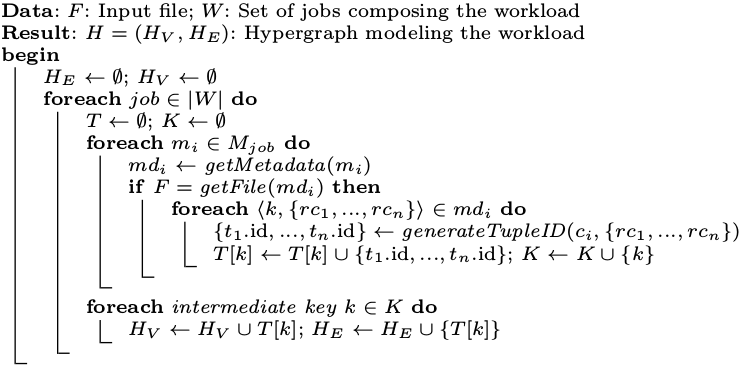
\includegraphics[width=1\textwidth, angle=0]{files/alg1}
	\caption[Pseudokód algoritmu pro Metadata Combination]
	{Pseudokód algoritmu pro Metadata Combination}\label{fig:alg1}
\end{figure} 

\subsection{Druhá fáze - Repartitioning}
Nyní, když je vygenerován hypergraf modelující rozložení dat v jednotlivých souborech, je na každý hypergraf aplikován min-cut k-way dělící algoritmus. Tento algoritmus má jako vstup hodnotu $k$ a hypergraf, ze kterého následně vygeneruje $k$ disjunktních podmožin vrcholů tak, aby byla minimalizována suma hran mezi uzly rozdílných podmnožin. Parametr $k$ je nastaven podle počtu bloků ve vstupním souboru. Po provedení tohoto algoritmu by měli být v jednotlivých vygenerovaných podmnožinách  seskupeny uzly generující stejný klíč. Následně se použijí tyto podmnožiny k vygenerování nových vstupních souborů, kde už jsou data seřazena tak, aby řádky generující stejný klíč byly maximálně seskupeny. Tímto nově vzniklým souborem je následně nahrazen starý vstupní soubor, který je smazán. Pseudokód algoritmu je uveden na obrázku. \ref{fig:alg2} V algoritmu je uvedená funkce $RR$, která reprezentuje funkci třídy $RecordReader$  použitou pro parsování vstupních souborů. Dále se v kódu oběvuje funkce $RW$ znamenající $RecordWriter$. Její funkce je inverzní k funkci $RecordReader$. V této části je výpočetně nejsložitější vykonání min-cut algoritmu. Min-cut algoritmus spadá do skupiny NP-Complete problémů. Existuje však několik aproximačních algoritmů, které byly navrženy k řešení tohoto problému. V tomto případě byl použit algoritmus \texttt{PATOH} \footnote{\texttt{http://bmi.osu.edu/$\sim$:umit/software.html}}

\begin{figure}\centering
	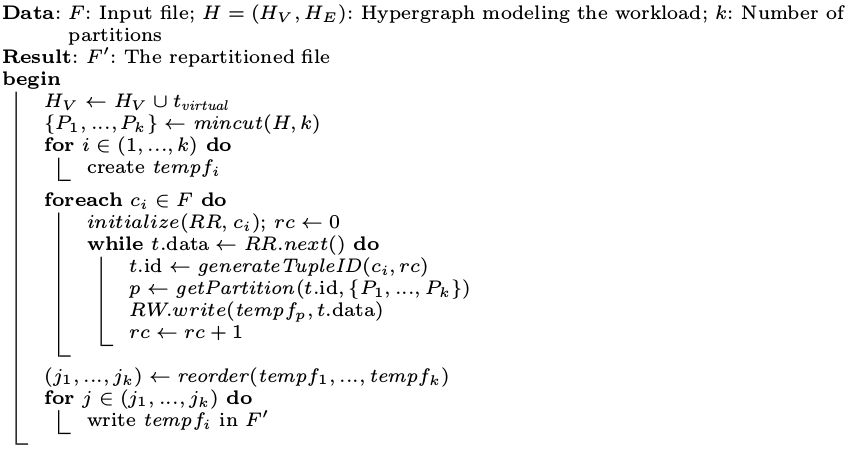
\includegraphics[width=1\textwidth, angle=0]{files/alg2}
	\caption[Pseudokód algoritmu pro Repartitioning]
	{Pseudokód algoritmu pro Repartitioning}\label{fig:alg2}
\end{figure} 

\subsection{Třetí fáze - Execution and scheduling}
K tomu, aby bylo možné plně využít výhody získané přeskupením záznamů v předchozích fázích, je zapotřebí maximalizovat data locality při plánování redukčních úloh. K tomuto účelu byl upraven algoritmus fairness-locality poskytnutý v \cite{cloudcom}, který pro každý pár key-value vypočítá skóre reprezentující poměr mezi vyvážeností vstupů do redukční fáze a lokací dat. Každý klíč je zpracován nezávisle pomocí greedy algoritmu. Pro každý klíč jsou pak možné uzly seřazeny podle jejich frekvence výskytu v sestupném pořadí (uzly s vyššími frekvencemi mají lepší data locality). Avšak namísto vybrání uzlu s maximální frekvencí se upřednostní uzel s lepším fairness-locality skore. To má za následek maximální vyvážení vstupů do redukčních fází.

V MapReduce frameworku je tedy nutné provést následující modifikace:

\begin{itemize}
  \item Upravení partitioning funkce tak, aby každému intermediate klíči přiřadila unikátní partition.
  \item Po dokončení mapovací části odeslat do master uzlu seznam s vygenerovanými intermediate klíči a jejich frekvencemi. Tato informace je přiložena k Heartbeat zpávě, která je odesílána po dokončení mapovací úlohy.
  \item Master přiřadí  intermediate klíč k redukční úloze na základě dodaných informací a zajístí tak maximální vyvážení a data-locality v redukční části výpočtu.
\end{itemize} 

\section{Testování a výsledky}
MR-Part byl implementován v Hodoop-1.0.4 a otestován na \texttt{Grid5000} \footnote{https://www.grid5000.fr/mediawiki/index.php/Grid5000:Home}. Jedná se o  rozsáhlou infrastrukturu složenou s rozdílných sítí s několika clustery výpočetních uzlů. Nutno podotknout, že tato infrastruktura není typická pro nasazení Hadoopu a vykonávání MapReduce úloh, především právě  kvůli nesourodosti clusterů v síti, jejich fyzické vzdálenosti a tím i kapacitně omezeném propojení. Částečně i proto bylo zrychlení zprácování tak znatelné. K testování byly využity datasety z \texttt{TPC-H} \footnote{http://www.tpc.org/tpch/www.grid5000.fr/mediawiki/index.php/Grid5000:Home}. 
\subsection{Výsledky}

\paragraph{Množství přenesených dat pro různé typy dotazů}. Při spustění několika různých úloh\texttt{TPC-H} \footnote{Implementace použitých dotazů: http://www.cs.duke.edu/starfish/mr-apps.html}.  na původních datasetech bylo v shuffle vázi přeneseno cca. 80\% dat. Po provedení dotazů na již upravených datech pak docházelo k přenosu dat  nižším než 10\% pro všechny provedené dotazy.

\paragraph{Množství přenesených dat v závislosti na velikosti clusteru}
Při provedení vybraného dotazu nad konfiguracemi systému s různým počtem clusterů nedocházelo k žádné výrazné změně v podílu přenesených dat. Jednalo se o konfigurace o 5 až 25 uzly v clusteru.

\paragraph{Časová náročnost dotazů}
Jak již bylo řečeno, časová náročnost je velmi vázaná na propustnost sítě. Bylo provedeno vykonání dotazů na různých šířkách pásma a výsledek byl očekávaný. Tedy čím pomalejší síť mezi výpočetními uzly, tím výraznější zrychlení při vykonávání dotazů.





\chapter{Návrh řešení pro HBase}
\section{Klíčová specifika HBase pro návrh řešení}
\subsection{Řazení záznamů v databázi}
\subsection{Automatický split a merge Hregionů}
\subsection{Fyzické uložení family column}

\section{Proces optimalizase}
\subsection{Monitoring}

\subsubsection{RecordReader Class}
\subsubsection{TableImputClass Class}
\subsubsection{Metadata file}

\subsection{Repartitioning}
\subsubsection{HyperGraph Class}
\subsubsection{PATOH Algoritmus}
\subsubsection{Repartioning Class}

\chapter{Implementace řešení}

\chapter{Testování a vyhodnocení měření}



\begin{conclusion}
	%sem napište závěr Vaší práce
\end{conclusion}

\bibliographystyle{csn690}
\bibliography{mybibliographyfile}

\appendix

\chapter{Seznam použitých zkratek}
% \printglossaries
\begin{description}
	\item[HDFS] Hadoop Distributed File System
	\item[REST] Representational State Transfer
	\item[CRUD] Create Read Update Delete
	\item[API] Application Programming Interface
	\item[SQL] Structured Query Language
	\item[NoSQL] Not only SQL
	\item[RDBMS] Relational DataBase Management System
	

\end{description}



\chapter{Obsah přiloženého CD}

%upravte podle skutecnosti

\begin{figure}
	\dirtree{%
		.1 readme.txt\DTcomment{stručný popis obsahu CD}.
		.1 exe\DTcomment{adresář se spustitelnou formou implementace}.
		.1 src.
		.2 impl\DTcomment{zdrojové kódy implementace}.
		.2 thesis\DTcomment{zdrojová forma práce ve formátu \LaTeX{}}.
		.1 text\DTcomment{text práce}.
		.2 thesis.pdf\DTcomment{text práce ve formátu PDF}.
		.2 thesis.ps\DTcomment{text práce ve formátu PS}.
	}
\end{figure}

\end{document}
